
\chapter{G\'en\'eralit\'es sur les fonctions} \label{fctgeneralites}
\minitoc

\fancyhead{}
\fancyfoot{} % efface les entêtes pr\'ec\'edentes
\fancyhead[LE,RO]{\footnotesize \em \rightmark}
		\fancyhead[RE,LO]{\scriptsize \em Seconde}
		\fancyfoot[RE]{\scriptsize \em \href{http://perpendiculaires.free.fr/}{http://perpendiculaires.free.fr/}}
		\fancyfoot[LO]{\scriptsize \em David ROBERT}
    \fancyfoot[LE,RO]{\textbf{\thepage}}
    
   % \sautpage
    

\section{Activit\'e d'introduction}\label{FonctionPbDIntro}
\subsection{Un probl\`eme}

\begin{tabular}{cc}
 \begin{minipage}[l]{0.25\linewidth}
  \begin{center}
\psset{xunit=0.25cm , yunit=0.25cm}
\begin{pspicture*}(-8.1,-1.4)(5.1,14.1)
\def\xmin{-5} \def\xmax{5} \def\ymin{-1.3} \def\ymax{14}

\def\F{1 2 div 4 x 2 exp sub 0.5 exp mul}
\psplot[linecolor=black,linestyle=solid,plotpoints=200]{-2}{2}{\F}
\def\G{0 1 2 div 4 x 2 exp sub 0.5 exp mul sub}
\psplot[linecolor=black,linestyle=solid,plotpoints=200]{-2}{2}{\G}
\def\H{12 1.5 4 div 16 x 2 exp sub 0.5 exp mul add}
\psplot[linecolor=black,linestyle=solid,plotpoints=200]{-4}{4}{\H}
\def\I{12 1.5 4 div 16 x 2 exp sub 0.5 exp mul sub}
\psplot[linecolor=black,linestyle=solid,plotpoints=200]{-4}{4}{\I}
\psline(0,0)(0,6)
\psline(-3.85,11.6)(0,6)(3.85,11.6)
\psline{<->}(-3.9,12)(3.9,12)
\rput(0,12.6){\small 8 cm}
\psline{<->}(-4.5,12)(-4.5,6)
\uput[l](-4.2,9){\small 6 cm}
\psdot(4,12)\rput[l](4.1,12){$A$}
\psdot(-4,12)\rput[ur](-4.1,12.3){$B$}
\psdot(0,6)\rput[l](0.2,5.9){$S$}

\end{pspicture*}\end{center}
 \end{minipage}&
 \begin{minipage}[l]{0.75\linewidth}
  Un verre \`a pied a une forme conique dont la base est un disque de 8\,cm de diam\`etre et de hauteur 6\,cm. Il repose sur une table parfaitement horizontale.
On d\'esire le remplir de fa\c con \`a ce qu'il contienne la moiti\'e de son volume maximal.
On recherche donc jusqu'\`a quelle hauteur il faut verser du liquide pour qu'il soit rempli \`a moiti\'e.
 \end{minipage}


\end{tabular}


\subsection{Travail pr\'eparatoire}

\emph{Ce travail est \`a faire \`a la maison.}


On appelle $h$ la hauteur \`a laquelle est vers\'ee le liquide.
\begin{enumerate}
	\item Entre quelles valeurs peut varier $h$ ?
	\item Quel est le volume maximal que peut contenir le verre ?
	\item Si on verse du liquide jusqu'\`a mi hauteur (3 cm) dans le verre, aura-t-on la moiti\'e du volume maximal du verre ?
	\item \label{fgq1} Calculer le rayon puis l'aire de la base puis le volume du liquide dans le verre lorsque $h=2$ cm, lorsque $h=3$ cm et lorsque $h=4$ cm.
	\item D\'eterminer le rayon puis l'aire de la base puis le volume du liquide dans le verre en fonction de $h$
(quelles formules de calcul permettent d'obtenir le rayon, l'aire de la base et le volume du liquide dans le verre, lorsque l'on conna\^it $h$ ?).
\end{enumerate}

\subsection{Utilisation du tableur comme calculateur}

\emph{Ce travail est \`a faire en salle informatique en groupe.}

\begin{enumerate}
	\item Cr\'eer la feuille de calcul suivante :
				\begin{center}
				\begin{tabular}{c|c|c|c|c|c}
				 &A&B &C &D &E  \\ \hline
				 1& & \multicolumn{2}{c|}{Volume du liquide} & & \\ \hline
				 2& & & & & \\ \hline
				 3& hauteur & rayon & aire de la base & VOLUME &  \\ \hline
				 4& & & & & \\ \hline
				 5& & & & & \\ \hline
				 6& & & & & \\ \hline
				\end{tabular}
				\end{center}
	\item Cr\'eer dans les cellules B4, C4, D4, et E4 les formules donnant, en fonction de la hauteur $h$, respectivement le rayon, l'aire de la base du cône et le volume du liquide dans le verre. \emph{Indication : $\pi$ s'obtient en entrant PI().}
	\item Contrôler les r\'esultats de la question \ref{fgq1} du travail pr\'eparatoire en entrant successivement les valeurs 2, puis 3 et enfin 4 dans la cellule A4 qui correspond \`a la hauteur.
	\item Parmi les valeurs enti\`eres de $h$, d\'eterminer de même celle pour laquelle le volume du liquide est le plus proche de la moiti\'e du volume du verre.
\end{enumerate}

\subsection{Cr\'eation d'un tableau}


\begin{enumerate}
	\item \begin{enumerate}
				\item S\'electionner le tableau cr\'e\'e pr\'ec\'edemment, puis le recopier (avec les menus Edition, Copier) sur une autre feuille de calcul du tableur.
				\item Entrer la valeur 0 dans la cellule A4, puis la formule =A4+1 dans la cellule A5. Recopier cette formule vers le bas de façon \`a obtenir les valeurs demand\'ees de la hauteur.
				\item S\'electionner alors les cellules B4 \`a D4 et, de même que pr\'ec\'edemment, les recopier vers le bas.
			\end{enumerate}
	\item On d\'esire plus de pr\'ecision.
				\begin{enumerate}
					\item Entrer la valeur 0 dans la cellule A4, puis la formule =A4+0,5 dans la cellule A5. Recopier cette formule vers le bas de façon \`a ce que les valeurs de la hauteur aillent de 0 \`a 6.
				\item S\'electionner alors les cellules B4 \`a D4 et, de même que pr\'ec\'edemment, les recopier vers le bas.
				\end{enumerate}
\end{enumerate}
\`A l'aide des r\'esultats obtenus, compl\'eter le tableau suivant :
\vspace{-1em}\begin{center}
\begin{tabular}{|c|*{13}{p{0.75cm}|}}
\hline
hauteur & 0 & 0,5 & 1 & 1,5 & 2 & 2,5 & 3 & 3,5 & 4 & 4,5 & 5 & 5,5 & 6 \\
\hline
VOLUME & & & & & & & & & & & & & \\
\hline
\end{tabular}
\end{center}

\subsection{Repr\'esentation graphique du volume en fonction de $h$}

\begin{enumerate}
	\item S\'electionner dans le tableau la colonne ''hauteur'' et la colonne ''VOLUME'' avec leurs titres.
\emph{Indication : pour s\'electionner deux colonnes (ou plus g\'en\'eralement des plages de cellules) non voisines, proc\'eder ainsi : s\'electionner la premi\`ere puis, en maintenant appuy\'ee la touche \emph{Ctrl} s\'electionner la seconde.}
	\item Cliquer sur l'icône correspondant \`a l'insertion d'un graphique. Essayer les diff\'erents types de repr\'esentations (un aperçu est propos\'e), puis en choisir un et se laisser guider par les indications de l'assistant graphique.
	\item \`A l'aide du graphique obtenu, donner une valeur arrondie au millim\`etre de la hauteur pour laquelle le volume est \'egal \`a la moiti\'e de celui du verre, ainsi qu'une valeur approch\'ee de ce volume.
\end{enumerate}

\subsection{Exploitation de la courbe repr\'esentative}

Vous trouverez en annexe la courbe obtenue avec le tableur en module qui donne le volume du liquide dans le verre en fonction de la hauteur de liquide dans le verre.

On note $V(h)$ le volume en fonction de la hauteur $h$. Ainsi $V (3) =12,566 \text{cm}^3$ car pour une hauteur de 3
cm, on peut lire graphiquement que le volume est de 12,566 $\text{cm}^3$.
\begin{enumerate}
	\item Pour quelle valeurs de $h$, peut-on d\'eterminer $V(h)$ ?
	\item Quel est le volume pour une hauteur de 5 cm ? \\
	Compl\'eter $V (5) = \ldots\ldots$ \\
	On dit que :
	\begin{itemize}
		\item 5 a pour image $\ldots\ldots$ par la fonction $V$ ; \\ $\ldots\ldots$ est l'image de 5 par la fonction $V$ ;
		\item $\ldots\ldots$ a pour ant\'ec\'edent 5 par la fonction $V$ ; \\ 5 est un ant\'ec\'edent de $\ldots\ldots$ par la fonction $V$.
	\end{itemize}
	\item Quel est le volume pour une hauteur de 2,5 cm ? \\
	Compl\'eter $V (2,5) = \ldots\ldots$ \\
	On dit que :
	\begin{itemize}
		\item 2,5 a pour image $\ldots\ldots$ par la fonction $V$ ;
		\item 2,5 est un ant\'ec\'edent de $\ldots\ldots$ par la fonction $V$.
	\end{itemize}
	\item Pour quelle hauteur le volume est-il de 70 $\text{cm}^3$ ? 50 $\text{cm}^3$ ? \\
	Compl\'eter :
	\begin{itemize}
	\item 70 a pour ant\'ec\'edent(s) $\ldots\ldots$ par la fonction $V$ ;
	\item 50 a pour ant\'ec\'edent(s) $\ldots\ldots$ par la fonction $V$.
	\end{itemize}
	\item
	\begin{enumerate}
		\item D\'eterminer l'image de 1, de 2, de 4 et de 6 par la fonction $V$.
		\item D\'eterminer les ant\'ec\'edents de 0, de 25, de 60 et de 80 par la fonction $V$.
		\item Peut-on d\'eterminer l'image de 13 par la fonction $V$ ? Pourquoi ?
		\item Peut-on d\'eterminer les ant\'ec\'edents de 120 par la fonction $V$ ?
		 Pourquoi ?
		\item R\'esoudre par lecture graphique :
			\begin{itemize}
				\item l'\'equation $V(h) = 75$.\\
Que signifie la r\'eponse \`a cette question ?
				\item l'in\'equation $V(h) > 50$.
			\end{itemize}
	\end{enumerate}
\end{enumerate}
%\sautpage
\subsection{Annexe}


\begin{center}
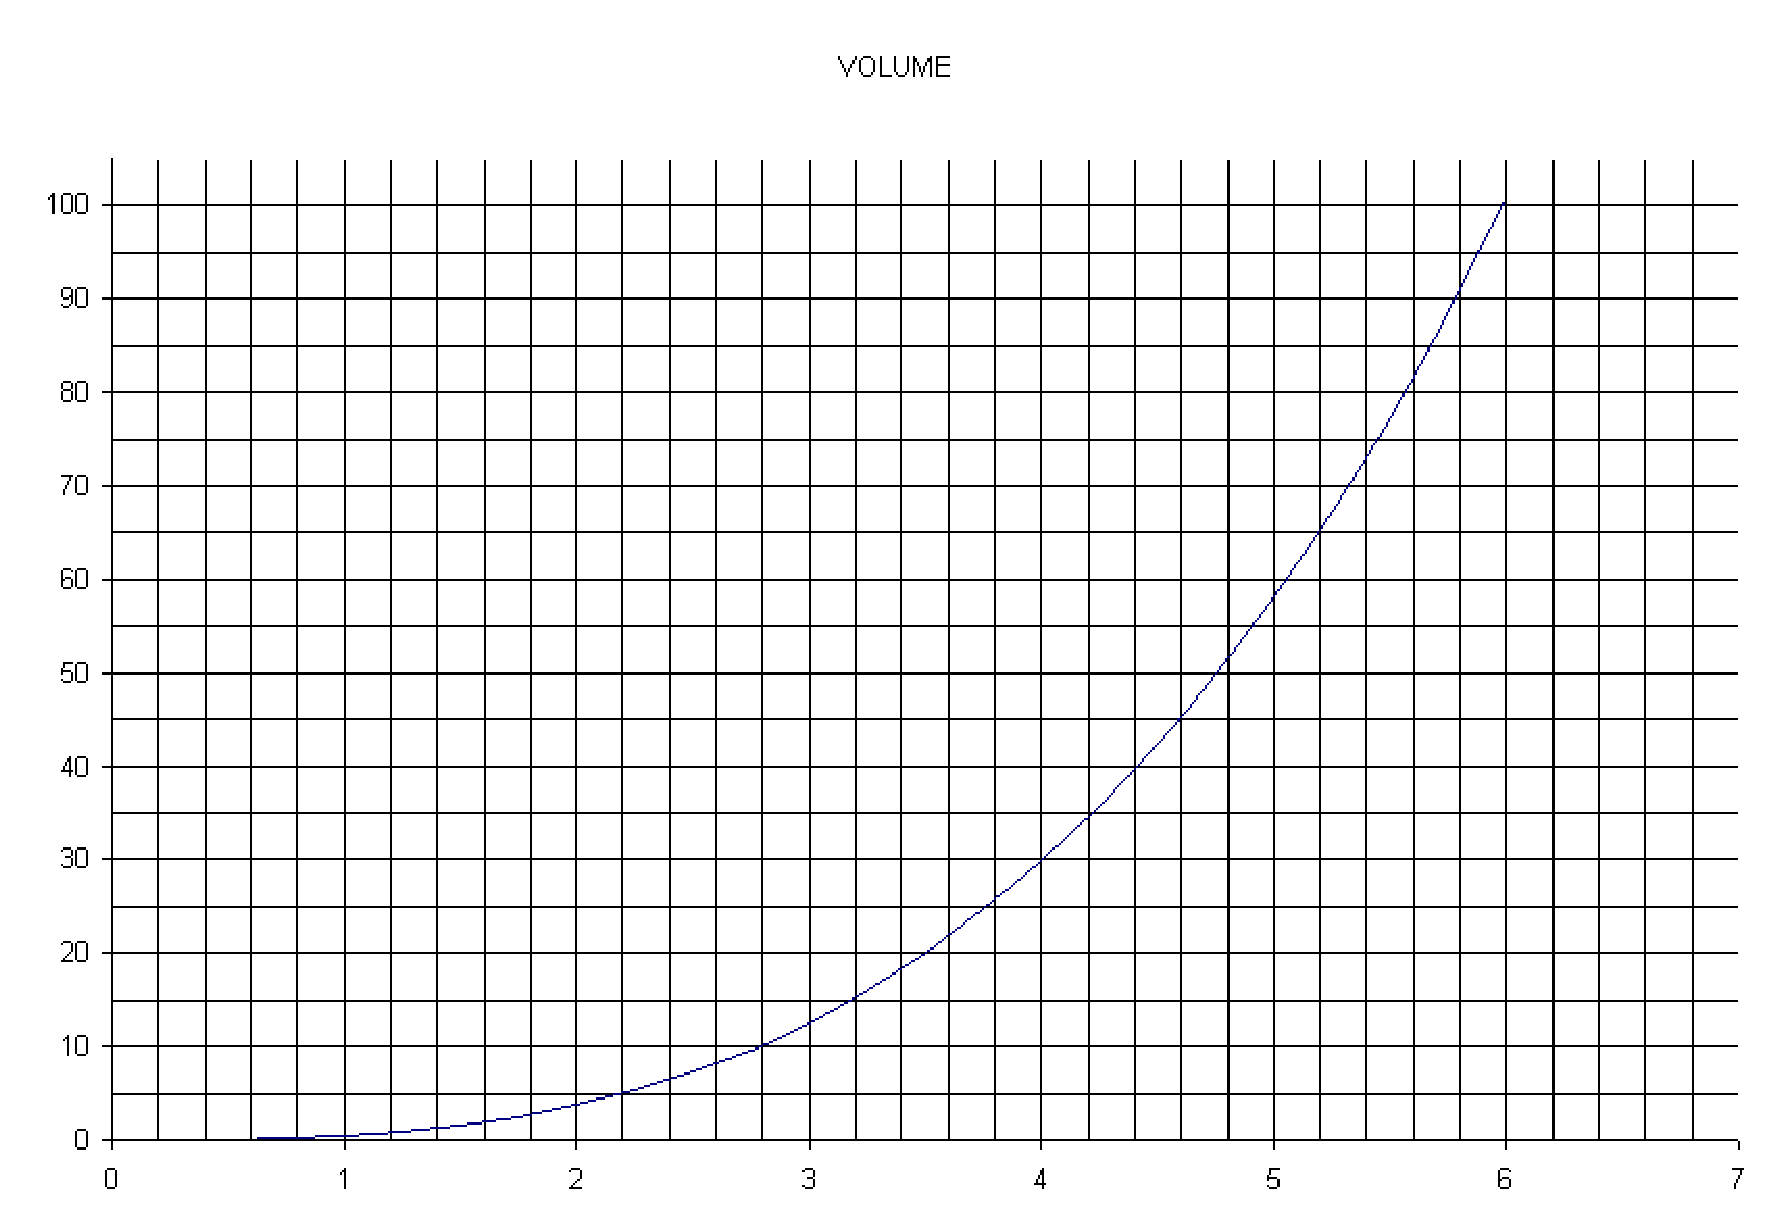
\includegraphics[scale=0.625]{./Graphiques/courbe.eps}\end{center}

%%%%%%%%%%%%%%%%%%%%%%%%%%%%%%%%%%%%%%%%%%%%%%%%%%%%
%%%%%%%%%%%%%%%%%%%%%%%%%%%%%%%%%%%%%%%%%%%%%%%%%%%

%%%%%%%%%%%%%%%%%%%%%%%%%%%%%%%%%%%%%%%%%%%%%%%%%%%\`u
%%%%%%%%%%%%%%%%%%%%%%%%%%%%%%%%%%%%%%%%%%%%%%%%%%%%

 \sautpage

\section{Premi\`eres notions (bilan et compl\'ements)}

\begin{definition}[Notion de fonction]
Une fonction est un proc\'ed\'e qui, \`a un \'el\'ement $x$ d'un ensemble de d\'epart, associe au plus un \'el\'ement $y$ d'un ensemble d'arriv\'ee.

On notera $f:x\mapsto y$ ou $f(x)=y$ qui se lit \og $f$ est la fonction qui \`a $x$ associe $y$ \fg..

On dit que $y$ est \emph{l'image} de $x$.

On dit que $x$ est \emph{un ant\'ec\'edent} de $y$.

\end{definition}

\begin{definition}[Ensemble de d\'efinition]
L'ensemble des r\'eels $x$ poss\'edant une image par une fonction num\'erique $f$ est appel\'e \emph{l'ensemble de d\'efinition de la fonction $f$}. On le note souvent $D_f$.
\end{definition}

\begin{definition}[Repr\'esentation graphique]
Dans un plan muni d'un rep\`ere, la \emph{repr\'esentation graphique} de la fonction $f$ est l'ensemble des points $M$ de coordonn\'ees $(x;y)$ du plan tels que :
\begin{itemize}
	\item L'abscisse $x$ de $M$ d\'ecrit l'ensemble de d\'efinition $D_f$ ;
	\item L'ordonn\'ee $y$ est l'image de $x$ par $f$. $y=f(x)$.
\end{itemize}

On note souvent $\mathcal{C}_f$ la repr\'esentation graphique de $f$. On dit que $\mathcal{C}_f$ a pour \'equation $y=f(x)$.

Si la courbe est d'un seul \og{} tenant \fg{} on parle  de \emph{courbe repr\'esentative} de la fonction $f$.
\end{definition}


\begin{rmq} L'\'equation permet de d\'eterminer si un point $A(x_A;y_A)$ appartient ou pas \`a cette courbe. En effet, un point appartient \`a la courbe si et seulement si ses coordonn\'ees v\'erifient l'\'equation de la courbe. On a alors : \[A\in\mathcal{C}_f\ssi y_A=f(x_A)\] \end{rmq}


Dans la pratique, pour les fonctions num\'eriques d\'efinies par une expression alg\'ebrique, pour esquisser une repr\'esentation graphique, on utilise souvent un tableau de valeurs.

\begin{tabular}{cc}
 \begin{minipage}[l]{0.55\linewidth}
  \begin{rmq} Une courbe ne repr\'esente pas toujours une fonction. Sur la figure ci-contre, par exemple, la courbe a plusieurs points ayant la même abscisse, comme $A(1,-1)$ et $B(1,3)$. Ce n'est donc pas la courbe repr\'esentative d'une fonction car alors 1 aurait plusieurs images.\end{rmq}
 \end{minipage}&
 \begin{minipage}[r]{0.45\linewidth}
\begin{center}
\psset{xunit=0.75cm , yunit=0.75cm}
\def\xmin{-2} \def\xmax{4} \def\ymin{-1.6} \def\ymax{3.6}
\begin{pspicture*}(\xmin,\ymin)(\xmax,\ymax)
\psset{xunit=0.75cm,yunit=0.75cm}
\psgrid[griddots=10,gridlabels=0pt,gridwidth=.3pt, gridcolor=black, subgridwidth=.3pt, subgridcolor=black, subgriddiv=1](0,0)(-2,-2)(4,4)
\psaxes[labels=all,labelsep=1pt, Dx=1,Dy=1]{->}(0,0)(\xmin,\ymin)(\xmax,\ymax)
\uput[dl](0,0){$O$}
%\pcline[linewidth=1pt]{->}(0,0)(1,0) \uput[d](0.5,0){\small $\vec \imath$}
%\pcline[linewidth=1pt]{->}(0,0)(0,1) \uput[l](0,0.5){\small $\vec \jmath$}
\pscircle(1,1){1.5}
\psdots[dotstyle=x](1,-1)(1,3)
\uput[d](1,-1){$A$}
\uput[u](1,3){$B$}
\end{pspicture*}
\end{center}
 \end{minipage}

\end{tabular}






%\sautpage

\subsubsection{Quelques conventions graphiques}
\begin{multicols}{3}
Lorsqu'un point $A$ sur la courbe est connu avec pr\'ecision, il est not\'e par une croix.
\begin{center}
\begin{pspicture*}(-0.5,-1)(2.5,3)
\pscurve(0,0)(0.5,-0.5)(1,1)(2,2.5)
\uput[u](0,0){$\mathcal{C}_f$}
\psdot[dotstyle=x](1,1)
\uput[dr](1,1){$A$}
\end{pspicture*}
\end{center}\sautcol
Lorsqu'un point $A$ est l'extr\'emit\'e de la courbe, il est not\'e par un gros point.
\begin{center}
\begin{pspicture*}(-0.5,-1)(2.5,3)
\pscurve(0,0)(0.5,-0.5)(1,1)(2,2.5)
\uput[u](0,0){$\mathcal{C}_f$}
\psdot(2,2.5)
\uput[dr](2,2.5){$A$}
\end{pspicture*}
\end{center}\sautcol
Lorsqu'un point $A$ \`a l'extr\'emit\'e de la courbe n'appartient pas \`a la courbe, il est not\'e par un \og demi-cercle \fg.
\begin{center}
\begin{pspicture*}(-0.5,-1)(2.5,3)
\pscurve{-(}(0,0)(0.5,-0.5)(1,1)(2,2.5)
\uput[u](0,0){$\mathcal{C}_f$}
%\psdot[(2,2.5)
\uput[dr](2,2.5){$A$}
\end{pspicture*}
\end{center}
\end{multicols}
\begin{multicols}{3}
Une courbe est donn\'ee dans une fenêtre ; s'il n'y a pas d'extr\'emit\'es, la courbe garde la même allure quand on la prolonge.
\begin{center}
\begin{pspicture*}(-0.5,-1)(2.5,3)
\pscurve(-0.3,0)(0.5,2)(1,1)(2,2.8)
\uput[u](1,1){$\mathcal{C}_f$}
\psline[linestyle=dotted](-0.1,0.5)(1.7,0.5)(1.7,2.2)(-0.1,2.2)(-0.1,0.5)
\end{pspicture*}
\end{center}
Une droite verticale en pointill\'es signifie que si l'on prolonge la courbe, elle ne coupe pas cette droite. Sur l'exemple ci-dessous, $a$ n'appartient pas \`a $D_f$.
\begin{center}
\begin{pspicture*}(-0.5,-1)(2.5,3)
\psaxes[labels=none,labelsep=1pt,Dx=5,Dy=5]{->}(0,0)(-0.5,-1)(2.5,3)
\psset{algebraic=true}
\psplot{0.6}{3}{1/(4*x-2)}
\psline[linestyle=dashed](0.5,-1)(0.5,3)
\uput[dl](0.5,0){$a$}
\end{pspicture*}
\end{center}
Une droite horizontale en pointill\'es signifie que si l'on prolonge la courbe, elle ne coupe pas cette droite.
\begin{center}
\begin{pspicture*}(-0.5,-1)(2.5,3)
\psaxes[labels=none,labelsep=1pt,Dx=5,Dy=5]{->}(0,0)(-0.5,-1)(2.5,3)
\psset{algebraic=true}
\psplot{-0.5}{3}{1+1/(x+1)}
\psline[linestyle=dashed](-0.5,1)(2.5,1)
\uput[ul](0,1){$b$}
\end{pspicture*}
\end{center}
\end{multicols}

%\sautpage






\section{R\'esolutions graphiques d'\'equations et d'in\'equations}


\subsection{R\'esolutions d'\'equations de la forme $f(x)=k$}

R\'esoudre l'\'equation $f(x)=k$ c'est d\'eterminer tous les ant\'ec\'edents \'eventuels d'un \'el\'ement $k$ de l'ensemble d'arriv\'ee, c'est-\`a-dire chercher tous les $x$ de l'ensemble de d\'epart tels que $f(x)=k$.

Une telle recherche peut se faire graphiquement \`a partir de la repr\'esentation graphique de la fonction $f$.




\begin{center}
\begin{tabular}{lc}
 \begin{minipage}[l]{0.6\linewidth}
 \begin{exemple*}
  Soit $f$ la fonction d\'efinie sur $\R$ par $f(x)=2x^2-9x+10$. On recherche les solutions de l'\'equation $f(x)=3$.

	On commence par tracer soigneusement la courbe repr\'esentative de $f$ et on obtient la repr\'esentation donn\'ee sur la figure ci-dessous.
		
		On cherche les points de la courbe ayant pour ordonn\'ee 3. Pour cela on peut tracer la droite d'\'equation $y=3$ et chercher les points d'intersection de cette droite avec la courbe de $f$.

		On obtient ici deux points $M_1(1;3)$ et $M_2\left(\frac{7}{2};3\right)$. Les solutions sont leurs abscisses : 1 et $\frac{7}{2}$.

		On \'ecrit : \og Les solutions de l'\'equation $f(x)=3$ sont $x=1$ ou $x=\frac{7}{2}$ car les points de la courbe de $f$ d'ordonn\'ee 3 ont pour abscisses 1 et $\frac{7}{2}$ \fg.
		\end{exemple*}
 \end{minipage}&
 \begin{minipage}[r]{0.35\linewidth}
  
		\begin{center}
 \psset{xunit=1cm,yunit=1cm}
		\begin{pspicture*}(-3.1,-2.1)(4.6,4.1)
\def\xmin{-3} \def\xmax{4.5} \def\ymin{-2} \def\ymax{4}

\psgrid[griddots=10,gridlabels=0pt,gridwidth=.3pt, gridcolor=black, subgridwidth=.3pt, subgridcolor=black, subgriddiv=1](0,0)(-3,-2)(4.5,4)
\psaxes[labels=all,labelsep=1pt, Dx=1,Dy=1]{->}(0,0)(\xmin,\ymin)(\xmax,\ymax)
\uput[dl](0,0){$O$}
\pcline[linewidth=1pt]{->}(0,0)(1,0) \uput[d](0.5,0){\small $\vec \imath$}
\pcline[linewidth=1pt]{->}(0,0)(0,1) \uput[r](0,0.5){\small $\vec \jmath$}
\psset{algebraic=true}
\psplot{\xmin}{\xmax}{2*(x-1)*(x-1)-5*(x-1)+3}
\uput[ul](2,1){$\mathcal{C}_f$}
\psline[linestyle=dashed](\xmin,3)(\xmax,3)
\uput[u](-2,3){$y=3$}
\uput[ur](1,3){$M_1$}
\uput[ul](3.5,3){$M_2$}
\psdots[dotstyle=x](1,3)(3.5,3)
\psline[linestyle=dashed]{->}(1,3)(1,0)
\psline[linestyle=dashed]{->}(3.5,3)(3.5,0)
\end{pspicture*}\end{center}
 \end{minipage}

\end{tabular}             \end{center}



%\sautpage

\subsection{R\'esolutions d'in\'equations de la forme $f(x)\leqslant k$}

Ces in\'equations peuvent se r\'esoudre graphiquement. On proc\`ede de la façon suivante :
\begin{itemize}
	\item on trace soigneusement $\mathcal{C}_f$ dan un rep\`ere (orthogonal) ;
	\item on trace la droite d'\'equation $y=k$ ;
	\item on recherche les points de la courbe situ\'es \emph{sous} la droite ;
	\item l'ensemble des solutions est constitu\'e des abscisses de ces points.
\end{itemize}

\begin{exemple*} Sur l'exemple pr\'ec\'edent, si l'on doit r\'esoudre $f(x)\leqslant 3$, apr\`es avoir trac\'e $y=3$ on constate que les points de la courbe situ\'es sous cette droite ont leurs abscisses comprises entre 0 et $\frac{5}{2}$.

Donc $f(x)\leqslant 3 \ssi x\in\left[0;\frac{5}{2}\right]$.
\end{exemple*}

\begin{rmq}~
\begin{itemize}
	\item On r\'esoud de la même mani\`ere les \'equations du type $f(x)\geqslant k$.

On retient alors les abscisses des points situ\'es \emph{au-dessus} de la droite d'\'equation $y=k$.

Dans l'exemple $f(x)\geqslant 3 \ssi x\in \left] -\infty ; 0 \right] \cup \left[\frac{5}{2} ; +\infty\right[$.
	\item De même pour les in\'equations strictes : $f(x)>k$ ou $f(x)<k$. On excluera alors les abscisses des points d'intersection de la courbe et de la droite.

	Dans l'exemple $f(x)<3 \ssi x\in \left]0;\frac{5}{2}\right[$.
\end{itemize}
\end{rmq}

\subsection{R\'esolutions d'\'equations de la forme $f(x)=g(x)$}

Cela revient \`a chercher les \'el\'ements de l'ensemble de d\'epart qui ont la même image par $f$ et par $g$.

Une telle recherche peut se faire graphiquement. On recherche alors les points des deux courbes repr\'esentatives ayant même abscisse et même ordonn\'ee, c'est-\`a-dire les points d'intersection des deux courbes. 

\begin{tabular}{cc}
 \begin{minipage}[l]{0.6\linewidth}
  \begin{exemple*}

Soit $f$ et $g$ les fonctions d\'efinies sur $\R$ par, respectivement, $f(x)=x^2-1$ et $g(x)=-0,5x^2+x+4$. R\'esoudre graphiquement l'\'equation $f(x)=g(x)$.

	On commence par tracer soigneusement les deux courbes repr\'esentatives et on obtient la repr\'esentation donn\'ee sur la figure ci-contre.
	
	On cherche les points d'intersection des deux courbes, ici $M_1$ et $M_2$, et les solutions de l'\'equation sont leurs abscisses dont les valeurs approximatives sont $-1,5$ et $2,2$.

		Les solutions sont donc $x\approx -1,5$ et $x\approx 2,2$.
\end{exemple*}
 \end{minipage}&
 \begin{minipage}[r]{0.35\linewidth}
  \psset{xunit=0.75cm,yunit=0.75cm}
		\begin{pspicture*}(-3.1,-2.1)(4.6,5.1)
\def\xmin{-3} \def\xmax{4.5} \def\ymin{-2} \def\ymax{5}

\psgrid[griddots=10,gridlabels=0pt,gridwidth=.3pt, gridcolor=black, subgridwidth=.3pt, subgridcolor=black, subgriddiv=1](0,0)(-3,-2)(4.5,5)
\psaxes[labels=all,labelsep=1pt, Dx=1,Dy=1]{->}(0,0)(\xmin,\ymin)(\xmax,\ymax)
\uput[dl](0,0){$O$}
\pcline[linewidth=1pt]{->}(0,0)(1,0) \uput[d](0.5,0){\small $\vec \imath$}
\pcline[linewidth=1pt]{->}(0,0)(0,1) \uput[r](0,0.5){\small $\vec \jmath$}
\psset{algebraic=true}
\psplot{\xmin}{\xmax}{x^2-1}
\psplot{\xmin}{\xmax}{-0.5*x^2+x+4}
\uput[u](1,1){$\mathcal{C}_f$}
\uput[dr](0,4){$\mathcal{C}_g$}
\uput[r](2.189,3.793){$M_2$}
\uput[l](-1.523,1.318){$M_1$}
\psdots[dotstyle=x](2.189,3.793)(-1.523,1.318)
\psline[linestyle=dashed]{->}(-1.523,1.318)(-1.523,0)
\psline[linestyle=dashed]{->}(2.189,3.793)(2.189,0)
\end{pspicture*}
	
 \end{minipage}


\end{tabular}

		

\subsection{R\'esolutions d'in\'equations de la forme $f(x)\leqslant g(x)$}

L\`a encore ces in\'equations peuvent se r\'esoudre graphiquement. On proc\`ede de la façon suivante :
\begin{itemize}
	\item on trace soigneusement $\mathcal{C}_f$ et $\mathcal{C}_g$ dans un rep\`ere (orthogonal) ;
	\item l'ensemble des solutions est constitu\'e des abscisses des points o\`u la courbe de $f$ est situ\'ee \emph{sous} celle de $g$.
\end{itemize}

\begin{exemple*} Sur l'exemple pr\'ec\'edent, si l'on doit r\'esoudre $f(x)\leqslant g(x)$, on constate que les points de la courbe de $f$ situ\'es sous celle de $g$ ont leurs abscisses comprises entre environ $-1,5$ et 2,2.

Donc $f(x)\leqslant g(x) \ssi x\in [-1,5;2,2]$. Ou bien $S=[-1,5;2,2]$.
\end{exemple*}

\begin{rmqs}~
\begin{itemize}
	\item On r\'esoud de la même mani\`ere les \'equations du type $f(x)\geqslant g(x)$.

On retient alors les abscisses des points de la courbe de $f$ situ\'es \emph{au-dessus} de celle de $g$.

Dans l'exemple $f(x)\geqslant g(x) \ssi x\in ] -\infty ; -1,5 ] \cup [2,2 ; +\infty[$.
	\item De même pour les in\'equations strictes : $f(x)>g(x)$ ou $f(x)<g(x)$. On excluera alors les abscisses des points d'intersection des deux courbes.

	Dans l'exemple $f(x)<g(x) \ssi x\in ]-1,5;2,2[$.
\end{itemize}
\end{rmqs}



%\sautpage



\sautpage

\section{Variations, extremums}


\subsection{Sens de variation}

Il s'agit de traduire math\'ematiquement qu'une fonction \og augmente \fg{} ou \og diminue \fg.

\begin{exemple*} Soit, par exemple, la fonction d\'efinie sur $[-3;3]$ par la courbe repr\'esentative donn\'ee sur la figure \ref{croissanceetdecroissance} \vpageref{croissanceetdecroissance}. On constate que lorsque $x\in[-3;1]$ , si $x$ augmente, $f(x)$ augmente aussi alors que lorsque $x\in[1;3]$, si $x$ augmente, $f(x)$ diminue.

C'est la d\'efinition math\'ematique de la croissance ou de la d\'ecroissance d'une fonction $f$.

\begin{figure}[h]
\centering
\caption{Croissance et d\'ecroissante}\label{croissanceetdecroissance}


\psset{xunit=1cm , yunit=1.25cm}
\begin{pspicture*}(-4.1,-1.1)(4.1,5.1)
\def\xmin{-4} \def\xmax{4} \def\ymin{-1} \def\ymax{5}
\psgrid[griddots=10,gridlabels=0pt,gridwidth=.3pt, gridcolor=black, subgridwidth=.3pt, subgridcolor=black, subgriddiv=1](0,0)(-4,-1)(4,5)
\psaxes[labels=all,labelsep=1pt, Dx=1,Dy=1]{-}(0,0)(\xmin,\ymin)(\xmax,\ymax)
\uput[dl](0,0){$O$}
\pcline[linewidth=1pt]{->}(0,0)(1,0) \uput[d](0.5,0){\small $\vec \imath$}
\pcline[linewidth=1pt]{->}(0,0)(0,1) \uput[r](0,0.5){\small $\vec \jmath$}
\psset{algebraic=true}
\psplot{-3}{3}{(-(x-1)^2+5)*0.25+3}
\psdots(3,3.25)(-3,0.25)
\uput[d](-1.5,0){$b$}
\psline[linestyle=dashed]{->}(-1.5,0)(-1.5,2.6875)
\psline[linestyle=dashed]{->}(-1.5,2.6875)(0,2.6875)
\uput[r](0,2.6875){$f(b)$}
\uput[d](-2.5,0){$a$}
\psline[linestyle=dashed]{->}(-2.5,0)(-2.5,1.1875)
\psline[linestyle=dashed]{->}(-2.5,1.1875)(0,1.1875)
\uput[r](0,1.1875){$f(a)$}
\uput[d](1.5,0){$u$}
\uput[d](2.5,0){$v$}
\psline[linestyle=dashed]{->}(1.5,0)(1.5,4.1875)
\psline[linestyle=dashed]{->}(1.5,4.1875)(0,4.1875)
\uput[l](0,4.1875){$f(u)$}
\psline[linestyle=dashed]{->}(2.5,0)(2.5,3.6875)
\psline[linestyle=dashed]{->}(2.5,3.6875)(0,3.6875)
\uput[l](0,3.6875){$f(v)$}
\end{pspicture*}
\end{figure}\end{exemple*}


\begin{definition}
Soit $f$ une fonction d\'efinie sur un intervalle $I$. On dit que $f$ est
\begin{itemize}
	\item \emph{croissante} sur $I$ si, pour tous r\'eels $a$ et $b$ de $I$, on a :\\
$\text{Si } a<b \text{ alors } f(a)\leqslant f(b).$
	\item \emph{d\'ecroissante} sur $I$ si, pour tous r\'eels $a$ et $b$ de $I$, on a :\\
$\text{Si } a<b \text{ alors } f(a)\geqslant f(b).$
	\item \emph{monotone} si elle n'est que croissante sur $I$ ou si elle n'est que d\'ecroissante sur $I$.
	\item \emph{constante} sur $I$ si, pour tous r\'eels $a$ et $b$ de $I$, on a : $f(a)=f(b)$.
\end{itemize}
\end{definition}


\begin{rmqs}~
\begin{itemize}
	\item Ces notions ne sont valables que sur \textbf{un intervalle} et pas sur une r\'eunion d'intervalles disjoints.
	\item Ant\'ec\'edents et images \'etant rang\'es dans le même ordre, on dit qu'une fonction croissante \emph{conserve} l'ordre.
	\item Ant\'ec\'edents et images \'etant rang\'es dans l'ordre inverse, on dit qu'une fonction d\'ecroissante \emph{inverse} l'ordre.
	\item On obtient les d\'efinitions d'une fonction \emph{strictement} croissante ou \emph{strictement} d\'ecroisante en remplaçant les in\'egalit\'es par des in\'egalit\'es strictes. Ainsi on dit que $f$ est strictement croissante sur $I$ si pour tous r\'eels $a$ et $b$ de $I$ on a : \\ $\text{Si } a<b \text{ alors } f(a)<f(b)$
	\item Une fonction est strictement monotone sur $I$ si elle est strictement croissante ou strictement d\'ecroissante sur $I$
\end{itemize}
\end{rmqs}

\subsection{Tableau de variations}

Ces r\'esultats peuvent se r\'esumer dans un tableau de variation, qui est une forme stylis\'ee de repr\'esentation o\`u l'on indique uniquement si la courbe monte, descend ou est stable. Dans la premi\`ere ligne on indique les valeurs importantes de $x$ et dans la seconde les variations de $f$.

\begin{exemple*} Dans l'exemple pr\'ec\'edent on obtient
$$\tabvar{%
\tx{x}&\tx{-3}&&\tx{1}&&\tx{3}\cr
\tx{f}&\txb{\approx 0,25}&\fm&\txh{\approx 4,25}&\fd&\txb{\approx 2,25}\cr
}$$
\end{exemple*}



\subsection{Extremums}

Les extremums, s'ils existent, sont les valeurs maximale et minimale qui sont \textbf{atteintes} par la fonction $f$ sur un intervalle donn\'e. Plus pr\'ecis\'ement :

\begin{definition}
Soit une fonction $f$ d\'efinie sur un intervalle $I$ et $x_0\in I$. On dit que
\begin{itemize}
	\item $f$ admet un \emph{maximum}, atteint en $x_0$ si, pour tout $x\in I$, $f(x)\leqslant f(x_0)$. Ce maximum est alors $f(x_0)$.
	\item $f$ admet un \emph{minimum}, atteint en $x_0$ si, pour tout $x\in I$, $f(x)\geqslant f(x_0)$. Ce minimum est alors $f(x_0)$.
\end{itemize}
Les maximum et minimum sont appel\'es les \emph{extremums}.
\end{definition}

%\begin{rmq} Un extremum doit être atteint par une valeur $x_0$. \end{rmq}

\begin{exemple*}
La fonction $f$ d\'efinie sur $\R$ par $f(x)=x^2+1$ n'admet pas $-1$ comme minimum.

En effet, si on a bien $f(x)\geqslant -1$ sur $\R$, il n'existe pas de $x_0$ tel que $f(x_0)=-1$.

Par contre 1 est bien le minimum de $f$ sur $\R$ car
\begin{itemize}
	\item $f(x)\geqslant 1$ pour tout $x\in\R$ \textbf{ET}
	\item $f(0)=1$
\end{itemize}

On dira donc : le minimum de $f$ sur $\R$ est 1 et il est atteint pour $x_0=0$.
\end{exemple*}

\sautpage

\section{Exercices et probl\`emes}

\subsection{Premi\`eres notions}

%\begin{multicols}{2}
%\begin{exo} Dire dans chacun des exemples ci-dessous quel est l'ensemble de d\'efinition, quelles sont les images possibles et si la fonction est num\'erique.
%\begin{enumerate}
%	\item \`A chaque \'el\`eve de la classe on associe la couleur de ses cheveux.
%	\item \`A chaque \'el\`eve de la classe on associe le nombre de ses fr\`eres et soeurs.
%	\item Pour un \'el\`eve donn\'e, \`a chaque moment de sa vie on associe la taille qu'il mesurait.
%	\item Soit $ABCD$ un rectangle dont un des côt\'es est fixe et mesure 6 cm et l'autre est variable et mesure $x$ cm. \\On d\'efinit la fonction $f$ de la façon suivante : \`a chaque $x$ possible, on associe $f(x)$, l'aire du rectangle $ABCD$.
%	\item La fonction $g$ d\'efinie par $g(x)=x^2+2x+3$.
%	\item La fonction $h$ d\'efinie par $h(x)=\frac{x^2+1}{x-1}$.
%	\item La fonction $i$ d\'efinie par $i(x)=\sqrt{x+2}$.
%\end{enumerate}
%\end{exo}
\begin{multicols}{2}
\begin{exo}
On d\'efinit $f$ et $g$, deux fonctions :
\begin{itemize}
	\item $f$ est la fonction qui \`a un nombre r\'eel $x$ associe le nombre obtenu en proc\'edant de la mani\`ere suivante : on ajoute $4$ au nombre, on \'el\`eve le r\'esultat obtenu au carr\'e, on retranche 16, on divise par le nombre de d\'epart et on retranche 6.
	\item $g:x\mapsto x^2-4$.
\end{itemize}
\begin{enumerate}
	\item Donner l'expression correspondant \`a $f$ puis simplifier cette expression.
	\item Quel r\'eel n'a pas d'image par $f$ ?
	\item Quelle est l'image de 3 par $g$ ?
	\item Quelle est l'image de $-1$ par $g$ ?
	\item Quels sont les ant\'ec\'edents \'eventuels de 12 par $g$ ?
	\item Quels sont les ant\'ec\'edents \'eventuels de $-5$ par $g$ ?
\end{enumerate}
\end{exo}

\sautcol

\begin{exo}
Vrai ou faux ? \emph{Corriger la phrase lorsqu'elle est fausse}.
\begin{enumerate}
	\item $f(-2) = 0$ signifie que l'image de 0 est $-2$
	\item $f(0) = 3$ signifie que la courbe de $f$ passe par le point $(0 ; 3)$
	\item $f(1) = 2$ signifie que l'ant\'ec\'edent de 1 est 2
	\item L'image de 2 par $f$ est $-3$ s'\'ecrit $f(2) = -3$
	\item Dire que $(5 ; 1)$ est un point de la courbe de $f$ s'\'ecrit $5 = f(1)$
	\item Par la fonction $g$, $-5$ est l'image de 3 s'\'ecrit $g(-5) = 3$
	\item 2 a pour image 0 par $f$ signifie que la courbe de $f$ traverse l'axe des abscisses en 2
	\item $f(4) = 0$ signifie que la courbe de $f$ traverse l'axe des abscisses au point $(4 ; 0)$
	\item 3 a pour image 5, signifie que 3 est l'image de 5
	\item 4 a pour ant\'ec\'edent 5 signifie que 5 est l'image de 4
\end{enumerate}
\end{exo}

\end{multicols}

%\sautpage

\begin{exo}\label{gf4courbes}
Vrai ou faux ? \emph{Justifier la r\'eponse lorsque c'est faux}.\\
Les courbes de la figure \ref{gf4courbesfig} \vpageref{gf4courbesfig} repr\'esentent des fonctions de la variable $x$.


\begin{figure}[!h]
 \centering
 \caption{Courbes de l'exercice \ref{gf4courbes}}\label{gf4courbesfig}
\begin{tabular}{cc}
\psset{xunit=1cm , yunit=0.5cm}
\begin{pspicture*}(-2.1,-2.1)(4.1,4.1)
\def\xmin{-2} \def\xmax{4} \def\ymin{-2} \def\ymax{4}
\psgrid[griddots=10,gridlabels=0pt,gridwidth=.3pt, gridcolor=black, subgridwidth=.3pt, subgridcolor=black, subgriddiv=1](0,0)(-2,-2)(4,4)
\psaxes[labels=all,labelsep=1pt, Dx=1,Dy=1]{->}(0,0)(\xmin,\ymin)(\xmax,\ymax)
\uput[dl](0,0){$O$}
\pcline[linewidth=1pt]{->}(0,0)(1,0) \uput[d](0.5,0){\small $\vec \imath$}
\pcline[linewidth=1pt]{->}(0,0)(0,1) \uput[l](0,0.5){\small $\vec \jmath$}
\psline(-2,3)(1,-1.5)(2,-1.5)(4,2)
\end{pspicture*}
&
\psset{xunit=1cm , yunit=0.5cm}
\begin{pspicture*}(-2.1,-2.1)(4.1,4.1)
\def\xmin{-2} \def\xmax{4} \def\ymin{-2} \def\ymax{4}
\psgrid[griddots=10,gridlabels=0pt,gridwidth=.3pt, gridcolor=black, subgridwidth=.3pt, subgridcolor=black, subgriddiv=1](0,0)(-2,-2)(4,4)
\psaxes[labels=all,labelsep=1pt, Dx=1,Dy=1]{->}(0,0)(\xmin,\ymin)(\xmax,\ymax)
\uput[dl](0,0){$O$}
\pcline[linewidth=1pt]{->}(0,0)(1,0) \uput[d](0.5,0){\small $\vec \imath$}
\pcline[linewidth=1pt]{->}(0,0)(0,1) \uput[l](0,0.5){\small $\vec \jmath$}
\psline(-2,3)(1,3)(1,1)(4,1)
\end{pspicture*}
\\
\psset{xunit=1cm , yunit=0.5cm}
\begin{pspicture*}(-2.1,-2.1)(4.1,4.1)
\def\xmin{-2} \def\xmax{4} \def\ymin{-2} \def\ymax{4}
\psgrid[griddots=10,gridlabels=0pt,gridwidth=.3pt, gridcolor=black, subgridwidth=.3pt, subgridcolor=black, subgriddiv=1](0,0)(-2,-2)(4,4)
\psaxes[labels=all,labelsep=1pt, Dx=1,Dy=1]{->}(0,0)(\xmin,\ymin)(\xmax,\ymax)
\uput[dl](0,0){$O$}
\pcline[linewidth=1pt]{->}(0,0)(1,0) \uput[d](0.5,0){\small $\vec \imath$}
\pcline[linewidth=1pt]{->}(0,0)(0,1) \uput[l](0,0.5){\small $\vec \jmath$}
\psline(-2,3)(4,3)
\end{pspicture*}
&
\psset{xunit=1cm , yunit=0.5cm}
\begin{pspicture*}(-2.1,-2.1)(4.1,4.1)
\def\xmin{-2} \def\xmax{4} \def\ymin{-2} \def\ymax{4}
\psgrid[griddots=10,gridlabels=0pt,gridwidth=.3pt, gridcolor=black, subgridwidth=.3pt, subgridcolor=black, subgriddiv=1](0,0)(-2,-2)(4,4)
\psaxes[labels=all,labelsep=1pt, Dx=1,Dy=1]{->}(0,0)(\xmin,\ymin)(\xmax,\ymax)
\uput[dl](0,0){$O$}
\pcline[linewidth=1pt]{->}(0,0)(1,0) \uput[d](0.5,0){\small $\vec \imath$}
\pcline[linewidth=1pt]{->}(0,0)(0,1) \uput[l](0,0.5){\small $\vec \jmath$}
\pscurve(-2,3)(-1,0)(0,-1)(2,1)(3.2,2)(3,3)
\end{pspicture*}
\end{tabular}
\end{figure}

\end{exo}

\sautpage

\begin{exo}\label{gf14}
Vrai ou faux ? \emph{Corriger la phrase lorsqu'elle est fausse}.\\
Les fonctions $f$ et $g$ sont repr\'esent\'ees sur la figure \ref{gf14fig} \vpageref{gf14fig}.
\begin{enumerate}
	\item La fonction $f$ est d\'efinie entre $-2$ et 6 inclus
	\item Les images par la fonction $f$ sont comprises entre $-1$ et 4 inclus
	\item La fonction $g$ est d\'efinie entre $-2$ exclu et 6 inclus
	\item Les images par la fonction g sont comprises entre 0 exclu et 3 inclus
\end{enumerate}



\begin{figure}[!h]
\centering
\caption{Courbes de l'exercice \ref{gf14}}\label{gf14fig}
\begin{tabular}{cc}
\psset{xunit=0.9cm , yunit=0.5cm}
\begin{pspicture*}(-3.1,-2.1)(6.1,5.1)
\def\xmin{-3} \def\xmax{6} \def\ymin{-2} \def\ymax{5}
\psgrid[griddots=10,gridlabels=0pt,gridwidth=.3pt, gridcolor=black, subgridwidth=.3pt, subgridcolor=black, subgriddiv=1](0,0)(-3,-2)(6,5)
\psaxes[labels=all,labelsep=1pt, Dx=1,Dy=1]{->}(0,0)(\xmin,\ymin)(\xmax,\ymax)
\uput[dl](0,0){$O$}
\pcline[linewidth=1pt]{->}(0,0)(1,0) \uput[d](0.5,0){\small $\vec \imath$}
\pcline[linewidth=1pt]{->}(0,0)(0,1) \uput[l](0,0.5){\small $\vec \jmath$}
\pscurve{*-(}(-2,2)(-1,3)(0,3.7)(0.5,3.9)(1,4)(2,3)(3,0)(4,-1)(5,0)(6,1)

\rput(3,2){$\mathcal{C}_f$}
\end{pspicture*}
&
\psset{xunit=0.9cm , yunit=0.5cm}
\begin{pspicture*}(-3.1,-2.1)(6.1,5.1)
\def\xmin{-3} \def\xmax{6} \def\ymin{-2} \def\ymax{5}
\psgrid[griddots=10,gridlabels=0pt,gridwidth=.3pt, gridcolor=black, subgridwidth=.3pt, subgridcolor=black, subgriddiv=1](0,0)(-3,-2)(6,5)
\psaxes[labels=all,labelsep=1pt, Dx=1,Dy=1]{->}(0,0)(\xmin,\ymin)(\xmax,\ymax)
\uput[dl](0,0){$O$}
\pcline[linewidth=1pt]{->}(0,0)(1,0) \uput[d](0.5,0){\small $\vec \imath$}
\pcline[linewidth=1pt]{->}(0,0)(0,1) \uput[l](0,0.5){\small $\vec \jmath$}
\pscurve{)-}(-2,0)(0,1)(1,2)(1.5,3.5)(1.8,5)
\pscurve{-*}(2.2,-2)(3,0)(4,1.5)(6,3)
\rput(1,3){$\mathcal{C}_g$}
\psline[linestyle=dashed](2,\ymin)(2,\ymax)
\end{pspicture*}
\end{tabular}
\end{figure}

\end{exo}

\begin{exo}\label{gf15}
Vrai ou faux ? \emph{Corriger la proposition lorsqu'elle est fausse}.
\begin{itemize}
	\item D'apr\`es la repr\'esentation graphique de la figure \ref{gf15fig} \vpageref{gf15fig} $D_f=[-4;2]$
	\item D'apr\`es la repr\'esentation graphique de la figure \ref{gf15fig} \vpageref{gf15fig} $D_g=]-\infty;3[\cup]3;5]$
\end{itemize}


\begin{figure}[!h]
\centering
\caption{Courbes de l'exercice \ref{gf15}}\label{gf15fig}
\begin{tabular}{cc}
\psset{xunit=1cm , yunit=0.66cm}
\begin{pspicture*}(-4.1,-2.1)(4.1,4.1)
\def\xmin{-4} \def\xmax{4} \def\ymin{-2} \def\ymax{4}
\psgrid[griddots=10,gridlabels=0pt,gridwidth=.3pt, gridcolor=black, subgridwidth=.3pt, subgridcolor=black, subgriddiv=1](0,0)(-4,-2)(4,4)
\psaxes[labels=all,labelsep=1pt, Dx=1,Dy=1]{->}(0,0)(\xmin,\ymin)(\xmax,\ymax)
\uput[dl](0,0){$O$}
\pcline[linewidth=1pt]{->}(0,0)(1,0) \uput[d](0.5,0){\small $\vec \imath$}
\pcline[linewidth=1pt]{->}(0,0)(0,1) \uput[l](0,0.5){\small $\vec \jmath$}
\pscurve{*-}(-4,0)(-3,-2)(0,0)(1,1)(4,1.8)
\psline[linestyle=dashed](0,2)(4,2)
\rput(-1.5,-1){$\mathcal{C}_f$}
\end{pspicture*}
&
\psset{xunit=1cm , yunit=0.66cm}
\begin{pspicture*}(-3.1,-2.1)(5.6,4.1)
\def\xmin{-3} \def\xmax{5.5} \def\ymin{-2} \def\ymax{4}
\psgrid[griddots=10,gridlabels=0pt,gridwidth=.3pt, gridcolor=black, subgridwidth=.3pt, subgridcolor=black, subgriddiv=1](0,0)(-3,-2)(5.5,4)
\psaxes[labels=all,labelsep=1pt, Dx=1,Dy=1]{->}(0,0)(\xmin,\ymin)(\xmax,\ymax)
\uput[dl](0,0){$O$}
\pcline[linewidth=1pt]{->}(0,0)(1,0) \uput[d](0.5,0){\small $\vec \imath$}
\pcline[linewidth=1pt]{->}(0,0)(0,1) \uput[l](0,0.5){\small $\vec \jmath$}
\pscurve(-3,3)(0,1.5)(1,1)(2,0)(2.8,-2)
\pscurve{-*}(3.2,-2)(4,1)(5,3)
\psline[linestyle=dashed](3,\ymin)(3,\ymax)
\uput[ur](1,1){$\mathcal{C}_g$}
\end{pspicture*}
\end{tabular}
\end{figure}
\end{exo}
%\sautpage


\begin{exo}[Avec la calculatrice]
La fonction $f$ est d\'efinie sur $[-1,5;2]$ par : $f(x)=2x^3-1,5x^2-3x$
\begin{enumerate}
	\item Compl\'eter le tableau de valeurs suivant :
	%\vspace{-1em}
	\begin{center}
\begin{tabular}{|*{9}{c|}}
\hline $x$ & $-1,5$ & $-1$ & $-0,5$ & 0 & 0,5 & 1 & 1,5 & 2 \\ \hline
$f(x)$ & & & & & & & & \\ \hline
\end{tabular}
\end{center}
\item Tracer la courbe repr\'esentative de $f$.
\end{enumerate}
\end{exo}

\begin{exo}[Avec la calculatrice]\label{uneautrecourbe}
La fonction $f$ est d\'efinie sur $[-3;3]$ par : $f(x)=x^2-3x+1$.\\
Apr\`es avoir dress\'e un tableau de valeurs de la fonction, tracer sa courbe repr\'esentative $\mathcal{C}_f$.

\end{exo}

%\end{multicols}



\sautpage

\subsection{R\'esolutions graphiques}

\begin{exo}
La fonction $f$ est d\'efinie sur $[-3;3]$ par : $f(x)=x^2-3x+1$.\\
$\mathcal{C}_f$, courbe repr\'esentative de $f$ a d\'ej\`a \'et\'e obtenue dans l'exercice \ref{uneautrecourbe}.
\begin{enumerate}
	\item \`A l'aide de la repr\'esentation graphique $\mathcal{C}_f$, avec la pr\'ecision permise par le graphique, r\'epondre aux question suivantes :
		\vspace{-1em}\begin{multicols}{2}
		  \begin{enumerate}
			\item Quelle est l'image de 2 ?
			\item Quelle est l'image de 3 ?
			\item Quelle est l'image de 4 ?
			\item Quels sont les ant\'ec\'edents de 1 ?
			\item Quels sont les ant\'ec\'edents de 2 ?
			\item Quels sont les ant\'ec\'edents de $-2$ ?
		\end{enumerate}
		\end{multicols}\vspace{-1em}
	\item R\'esoudre graphiquement les \'equations et in\'equations suivantes :
\vspace{-1em}\begin{multicols}{3}\begin{enumerate}
	\item $f(x)=3$ ;
	\item $f(x)=-1,5$ ;
	\item $f(x)\geqslant -1$ ;
	\item $f(x)<4$ ;
	\item $f(x)>-3$ ;
	\item $f(x)<-2$.
\end{enumerate}\end{multicols}\vspace{-1em}
\item D\'eterminer graphiquement le signe de $f(x)$ selon les valeurs de $x$.
\end{enumerate}
\end{exo}

%\sautpage

\begin{exo}
Une fonction $f$, d\'efinie sur $\R$, est donn\'ee par sa courbe repr\'esentative $\mathcal{C}$ :
\begin{multicols}{2}
\begin{center}\small
\psset{xunit=1,yunit=1}
\begin{pspicture*}(-2.6,-2.1)(5.1,3.1)
\def\xmin{-2.5} \def\xmax{5} \def\ymin{-2} \def\ymax{3}
\psset{xunit=0.1cm,yunit=0.1cm}
\psgrid[griddots=15,gridlabels=0pt,gridwidth=.3pt, gridcolor=gray, subgridwidth=.3pt, subgridcolor=gray, subgriddiv=1](0,0)(-25,-20)(50,30)
\psset{xunit=1cm , yunit=1cm}
\psaxes[labels=all,labelsep=1pt, Dx=1,Dy=1]{->}(0,0)(\xmin,\ymin)(\xmax,\ymax)
\uput[dl](0,0){$0$}
\pcline[linewidth=1pt]{->}(0,0)(1,0) \uput[d](0.5,0){\small $\vec i$}
\pcline[linewidth=1pt]{->}(0,0)(0,1) \uput[l](0,0.5){\small $\vec j$}
\pscurve(-2.3,-2)(-2,-1)(-1.5,1.5)(-1,3)(-0.5,2.5)(0,1)(0.2,0)(0.5,-1)(1,-1.5)(1.5,-1)(2,0)(2.5,1)(3,1.5)(4,2)(5,2.3)
\psline[linestyle=dashed](0,2.5)(\xmax,2.5)
\psdots[dotstyle=x](-2,-1)(-1.5,1.5)(-1,3)(-0.5,2.5)(0,1)(0.5,-1)(1,-1.5)(1.5,-1)(2,0)(2.5,1)(3,1.5)(4,2)
\end{pspicture*}
\end{center}\normalsize

\sautcol

Avec la pr\'ecision permise par le graphique, r\'esoudre :
%\vspace{-1em}
%\begin{multicols}{2}
\begin{enumerate}
	\item Les \'equations suivantes :
		\vspace{-1em}
		\begin{multicols}{2}\begin{enumerate}
			\item $f(x) = 1$ ;
			\item $f(x) = 0$ ;
			\item $f(x) = -1$ ;
			\item $f(x) = 2$.
		\end{enumerate}\end{multicols}
		%\vspace{-1em}
%\sautcol
	\item Les in\'equations suivantes :
		\vspace{-1em}
		\begin{multicols}{2}\begin{enumerate}
			\item $f(x)\geqslant 1$ ;
			\item $f(x)\geqslant 0$ ;
			\item $f(x)<-1$ ;
			\item $f(x)>2$.
		\end{enumerate}\end{multicols}
		\vspace{-1em}
	\item D\'eterminer graphiquement le signe de $f(x)$ selon les valeurs de $x$.

\end{enumerate}\end{multicols}
%\vspace{-1em}
\end{exo}

\medskip

\begin{multicols}{2}

\begin{exo}\label{gfunecourbe}
La courbe $\mathcal{C}$ de la figure ci-dessous %\ref{gfunecourbefig} \vpageref{gfunecourbefig} 
repr\'esente une fonction $f$ et le segment de droite $\mathcal{D}$ repr\'esente une fonction $g$.

%\begin{figure}[hbtp]
% \centering
% \caption{Figure de l'exercice \ref{gfunecourbe}}\label{gfunecourbefig}


\begin{center}
\psset{xunit=0.375cm , yunit=0.33cm}
\def\xmin{-9} \def\xmax{12} \def\ymin{-3} \def\ymax{11}
\begin{pspicture*}(\xmin,\ymin)(\xmax,\ymax)
\psgrid[griddots=10,gridlabels=0pt,gridwidth=.3pt, gridcolor=black, subgridwidth=.3pt, subgridcolor=black, subgriddiv=1](0,0)(\xmin,\ymin)(\xmax,\ymax)
\psaxes[labels=all,labelsep=1pt, Dx=5,Dy=5]{-}(0,0)(\xmin,\ymin)(\xmax,\ymax)
\uput[dl](0,0){$O$}
\pcline[linewidth=1pt]{->}(0,0)(1,0) \uput[d](0.5,0){\small $\vec \imath$}
\pcline[linewidth=1pt]{->}(0,0)(0,1) \uput[l](0,0.5){\small $\vec \jmath$}
\pscurve{*-*}(-8,1)(-5,3)(-3,5)(-1,6)(0,5)(1,3)(2,0)(4,-2)(7,0)(9,3)(11,6)
\psdots[dotstyle=x](-5,3)(-3,5)(-1,6)(0,5)(1,3)(2,0)(4,-2)(7,0)(9,3)
\psdots[dotstyle=*](-8,7.5)(11,-2)
\uput[dr](10,5){$\mathcal{C}$}
\uput[ur](-6,7){$\mathcal{D}$}
\psplot[linestyle=dashed,algebraic=true]{-8}{11}{-0.5*x+3.5}
\end{pspicture*}\end{center}

%\end{figure}

\sautcol

\begin{enumerate}
	\item R\'esoudre graphiquement les \'equations :
		\vspace{-1em}\begin{multicols}{2}\begin{enumerate}
			\item $f(x) = 3$ ;
			\item $f(x) = -2$ ;
			\item $f(x) = 0$ ;
			\item $f(x) = 6$.
		\end{enumerate}\end{multicols}
	\item R\'esoudre graphiquement les in\'equations :
		\begin{enumerate}
			\item $f(x)\leqslant 0$ ;
			\item $f(x) \geqslant 3$ ;
			\item $f(x)>5$.
		\end{enumerate}

	\item R\'esoudre graphiquement :
			\begin{enumerate}
				\item $f(x) = g(x)$ ;
				\item $f(x) < g(x)$.			\end{enumerate}
		\item Donner le signe de $f(x)$ suivant les valeurs de $x$.
\end{enumerate}
\end{exo}\end{multicols}

%\sautpage

\begin{multicols}{2}

\begin{exo}[Avec la calculatrice]
On consid\`ere les fonctions $f$ et $g$ d\'efinies sur $\R$ par : $f(x)=x^3$ et $g(x)=3x-2$.
 \begin{enumerate}
			\item Tracer soigneusement les repr\'esentations graphiques $\mathcal{C}_f$ et $\mathcal{C}_g$ de $f$ et $g$ sur l'intervalle $[-2;2]$.
			\item R\'esoudre graphiquement l'in\'equation $f(x)\leqslant 1$.
			\item D\'eterminer graphiquement les solutions de l'\'equation $f(x)=g(x)$.
 \end{enumerate}
\end{exo}

\sautcol

\begin{exo}[Avec la calculatrice]
Les fonctions $f$ et $g$ sont d\'efinies sur $[-2;2]$ par : $f(x)=x^3$ et $g(x)=1-x$.
\begin{enumerate}
	\item Tracer sur une calculatrice graphique les repr\'esentations graphiques $\mathcal{C}_f$ et $\mathcal{C}_g$ de $f$ et de $g$.
	\item En d\'eduire le nombre de solutions de l'\'equation $x^3+x-1=0$.
	\end{enumerate}
\end{exo}

\end{multicols}

\subsection{R\'esolutions calculatoires}
%\section{Technologie}
\begin{multicols}{2}
\begin{exo}
Soit la fonction $f$ d\'efinie sur $\R$ par : \\$f(x)=2x^2+x+3$.
\begin{enumerate}
	\item Calculer les valeurs exactes de $f(x)$ pour les valeurs de $x$ suivantes :
	  \vspace{-1em}\begin{multicols}{3}
	  \begin{itemize}
	    \item 0 ;
	    \item 1 ;
	    \item $-2$ ;
	    \item $\sqrt{2}$ ;
	    \item $1+\sqrt{3}$ ;
	    \item $2-\sqrt{5}$.
	   \end{itemize}
	  \end{multicols}\vspace{-1em}
	\item R\'esoudre $f(x)=3$.
\end{enumerate}
\end{exo}

\begin{exo}
Soit $f$ la fonction d\'efinie sur $\R$ par :\\ $f(x)=2x^2-5x+3$. \\R\'esoudre $f(x)=3$.
\end{exo}

\begin{exo} Soit $f$ la fonction d\'efinie sur $\R$ par : $f(x)=4x^2-4x+1$. On cherche \`a r\'esoudre, par le calcul, l'\'equation $f(x)=9$.
%\vspace{-1em}\begin{multicols}{2}
\begin{enumerate}
	\item Factoriser $f(x)$.
	\item R\'esoudre $f(x)=9$.
\end{enumerate}% \end{multicols}\vspace{-1em}
\end{exo}



\begin{exo}
	Soit $f$ et $g$ les fonctions d\'efinies sur $\R$ par, respectivement, $f(x)=x^2-1$ et $g(x)=-x^2+2$. \\ R\'esoudre par le calcul l'\'equation $f(x)=g(x)$.
\end{exo}


\begin{exo}
On consid\`ere les fonctions $f$ et $g$ d\'efinies sur $\R$ par : $f(x)=x^3$ et $g(x)=3x-2$. On cherche \`a r\'esoudre, par le calcul, l'\'equation $f(x)=g(x)$.
		\begin{enumerate}
			\item D\'evelopper $(x-1)^2(x+2)$.
			\item En d\'eduire les solutions de l'\'equation $x^3-3x+2=0$.
			\item En d\'eduire les solutions de l'\'equation $f(x)=g(x)$.
		\end{enumerate}
\end{exo}



%

\begin{exo}
On consid\`ere la fonction $f$ d\'efinie pour tout $x\in\R$ par : $f(x)=x(x-2)$. On cherche \`a trouver, par le calcul, le minimum de $f(x)$.
%\vspace{-1em}\begin{multicols}{2}
\begin{enumerate}
	\item D\'emontrer que $f(x)=(x-1)^2-1$.
	\item En d\'eduire le minimum de $f(x)$.
\end{enumerate}%\end{multicols}\vspace{-1em}
\end{exo}

\end{multicols}

\sautpage


\subsection{Variations, extremums}

\begin{multicols}{2}

\begin{exo}\label{fonctionsvar1}
On consid\`ere la fonction $f$ dont on donne la repr\'esentation $\mathcal{C}$ sur la figure \ref{fonctionsvar1fig} \vpageref{fonctionsvar1fig} (en deux parties).\\
Indiquer son ensemble de d\'efinition et dresser son tableau de variations.

\end{exo}
%\sautpage


\begin{exo}[Avec une calculatrice]
On consid\`ere la fonction $f$ d\'efinie par : $f(x)=2x\sqrt{4-x^2}$.
\`A l'aide d'une calculatrice graphique :
\begin{enumerate}
	\item conjecturer l'ensemble de d\'efinition de $f$ ;
	\item conjecturer quels sont les extremums de $f$ sur son ensemble de d\'efinition ;
	\item dresser le tableau des variations de $f$.
\end{enumerate}
\end{exo}


%\sautcol


\begin{exo}
Tracer une courbe repr\'esentative d'une fonction $f$ sachant que :
%\vspace{-1em}\begin{multicols}{2}
\begin{itemize}
\item le tableau des variations de $f$ est le suivant :$$\tabvar{%
\tx{x}&&&\tx{0}&&\tx{3}&&\tx{~}\cr
\tx{f}&\txb{1}&\fm&&\fd&&\fm&\cr
}$$
	\item 1 a pour ant\'ec\'edents, par la fonction $f$, $-2$ et 1,5 ;
	\item $f(x)=0$ a pour solutions $x=2$ ou $x=4$ ;
	\item $f(-1)=2$ ;
	\item $-1$ est l'image de 3 ;
	\item $D_f=[-2;4]$ ;
	\item le maximum de $f$ est 3 ;
	
\end{itemize}%\end{multicols}
\end{exo}



\sautcol

\begin{exo}
On donne le tableau des variations d'une fonction $f$ :$$\tabvar{%
\tx{x}&\tx{-5}&&\tx{-3}&&\tx{0}&&\tx{1}&&\tx{8}\cr
\tx{f}&\txh{3}&\fd&\txb{0}&\fm&\txh{1}&\fdh&\tx{0}&\fdb&\txb{-2}\cr
}$$
%\vspace{-4em}\begin{multicols}{2}
\begin{enumerate}
	\item S'il est possible de r\'epondre, compl\'eter par \og < \fg, \og > \fg{} ou \og = \fg. Sinon mettre une croix.
\begin{itemize}
 \item $f(-1)$  $\ldots\ldots$  $f(-2)$ 
 \item $f(-3)$  $\ldots\ldots$  $f(1)$ 
 \item $f(-1)$  $\ldots\ldots$  $1$ 
 \item $f(-2)$ $\ldots\ldots$  $f(0,5)$
 \item $f(-2)$  $\ldots\ldots$  $f(1,5)$
 \item $f(4)$  $\ldots\ldots$  $f(2)$
 \item $4$  $\ldots\ldots$ $f(-4)$
 \end{itemize}

\item R\'esoudre, lorsque c'est possible, les in\'egalit\'es suivantes :
\vspace{-1em}\begin{multicols}{2}\begin{enumerate}
	  \item $f(x)\geqslant 0$ ;
	  \item $f(x)=1$ ;
	  \item $f(x)<-1$ ;
	  \item $f(x)<0$.
  \end{enumerate}\end{multicols}
	\item Dire, si c'est possible, quel est le maximum de la fonction et quel est son minimum.
\end{enumerate}%\end{multicols}
\end{exo}
\end{multicols}
%M\end{multicols}



\begin{figure}[!h]
 \centering
 \caption{Figure de l'exercice \ref{fonctionsvar1}}\label{fonctionsvar1fig}

\psset{xunit=0.75cm , yunit=0.75cm}
\begin{pspicture*}(-6.1,-2.1)(14.1,6.1)
\def\xmin{-6} \def\xmax{14} \def\ymin{-2} \def\ymax{6}
\psgrid[griddots=10,gridlabels=0pt,gridwidth=.3pt, gridcolor=black, subgridwidth=.3pt, subgridcolor=black, subgriddiv=1](0,0)(-6,-2)(14,6)
\psaxes[labels=all,labelsep=1pt, Dx=1,Dy=1]{-}(0,0)(\xmin,\ymin)(\xmax,\ymax)
\uput[dl](0,0){$O$}
\pcline[linewidth=1pt]{->}(0,0)(1,0) \uput[d](0.5,0){\small $\vec i$}
\pcline[linewidth=1pt]{->}(0,0)(0,1) \uput[l](0,0.5){\small $\vec j$}
\pscurve(-5,-1)(-4,0)(-3,3)(-2,4)(0,3)(4,0)(5,-2)
\psdot(-5,-1)
\psdots[dotstyle=x](-4,0)(-3,3)(-2,4)(0,3)(4,0)(7,0)(8,3)(10,5)(12,3)
\pscurve(6.5,-2)(7,0)(8,3)(10,5)(12,3)(14,2.2)
\psline[linestyle=dashed](6,-2)(6,6)
\psline[linestyle=dashed](9,2)(14,2)
\end{pspicture*}
\end{figure}







%\sautpage

